\chapter[2019 March]{March 2019}

\section[2019/03/02]{Tuesday, 1 March 2019}
\label{sec:somewhere}

\subsection{This is a sample heading, typically activity related}

Some normal text....

\subsection{Approach: Lab book}

Some normal text....

\begin{slantnote}
  Keeping a lab notebook is generally considered best practice, both for
  engineering work and also research projects such as this. A paper based
  approach is however less than ideal as the resultant work cannot be
  easily searched. For work of this nature it has further disadvantages
  with respect to figures, plots and code fragments being harder to manage
  given that all three are to be generated automatically.

  A ``year+month'' based hierarchy was decided on in order to balance the
  complexity of organisation and the level of nesting. For the cases where
  additional files must be included. As a result of the nesting however the
  \LaTeX\ \texttt{$\backslash$input} command must be used to handle the
  inclusion.
\end{slantnote}

Some normal text....

\pendsign

\section[2019/03/03]{Thursday, 3 March 2019}

\subsection{Research Ideas}

\begin{compactitem}
\item Idea 1... testing acronym \ac{EM}
\item Idea 2... testing index \bidx{SLAM}
\item Idea 3... testing href and reference
\href{http://en.wikipedia.org/wiki/David_Marr_(neuroscientist)}{David Marr}
\index{Marr, David}~\cite{marr_aa_2010}
\end{compactitem}

\todoredefined{Should do a search to identify any relevant ... }

\EquRef{eqn:example} shows an example of a numbered equation.
\begin{equation}
  \Delta w_{i,j} = \alpha a_i \Delta[j]  \label{eqn:example}
\end{equation}
A subsection a subsection a subsection a subsection a subsection a
subsection a subsection a subsection a subsection a subsection a
subsection a subsection a subsection a subsection a subsection.
\nocite{dellaert_spieits_1997}

\FigRef{fig:example} shows an example of a figure.
\begin{figure}[!ht]
  \centering
  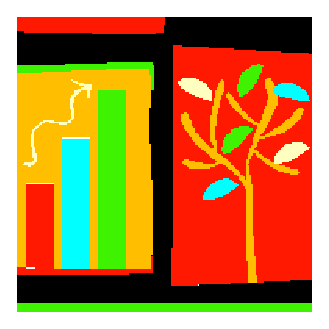
\includegraphics[width=0.4\linewidth]{figures/figure1}
  \caption{This is a figure caption}
  \label{fig:example}
\end{figure}

Third theme of literature study third theme of literature study third
theme of literature study third theme of literature study. See
\SecRef{sec:somewhere} for more information.

\subsection{Example of tables}

\TabRef{tab:eai732sch} shows an example of a table, extracted from the EAI732
study guide.
\begin{table}
  \centering
  \caption{Example table -- EAI732 Schedule}
  \label{tab:eai732sch}
    \begin{tabular}{ !{\vrule width 1.1pt}
                    c!{\vrule width 1pt}
                    c!{\vrule width 1pt}
                    c!{\vrule width 1pt}
                    p{8.6cm}!{\vrule width 1pt}}
    \noalign{\hrule height 1pt}
    \cellcolor[gray]{0.9} \textbf{Week} &
    \cellcolor[gray]{0.9} \textbf{Date} &
    \cellcolor[gray]{0.9} \textbf{Theme} &
    \cellcolor[gray]{0.9} \textbf{Required reading / Assignment due date }
    \\ \noalign{\hrule height 1pt}
    1     &   2 Feb --   8 Feb & 1 & Introduction - Bishop Chapter 1.
    \\ \hline
    2     &   9 Feb --  15 Feb & 1 & Probability Distributions - Bishop Chapter 2.
    \\ \hline
    3     &  16 Feb --  22 Feb & 1 & Regression \& Classification - Bishop Chapter 3 \& 4
    \\ \hline
    4     &  23 Feb --   1 Mar & 1 & Mixture Models and EM - Bishop Chapter 9.
    \\ \hline
    5     &   2 Mar --   8 Mar & 1 &
    \\ \hline
    6     &   9 Mar --  15 Mar & 2 & Neural Networks - Bishop Chapter 5. \\
            &                    &   & \textbf{Block 1} \\
            &                    &   & \textsl{Assignment 1 (due 9 March)}.
    \\ \hline
    7     &  16 Mar --  22 Mar & 2 &
    \\ \hline
    8     &  23 Mar --  29 Mar & 2 & Optimisation and Heuristic Algorithms.
    \\ \hline
    9     &  30 Mar --   5 Apr & 2 & \textbf{\emph{Recess}}.
    \\ \hline
    10    &   6 Apr --  12 Apr & 2 & \textbf{\emph{Recess}}.
    \\ \hline
    11    &  13 Apr --  19 Apr & 3 & Kernel Methods - Bishop Chapter 6. \\
            &                    &   & \textsl{Assignment 2 (due 13 April)}.
    \\ \hline
    12    &  20 Apr --  26 Apr & 3 & Support Vector Machines - Bishop Chapter 7.
    \\ \hline
    13    &  27 Apr --   3 May & 3 & \textbf{\emph{Recess}}.
    \\ \hline
    14    &   4 May --  10 May & 3 & Graphical Methods - Bishop Chapter 8. \\
            &                    &   & \textbf{Block 2}
    \\ \hline
    15    &  11 May --  17 May & 3 &
    \\ \hline
    16    &  18 May --  24 May & 4 & Sampling Methods - Bishop Chapter 11. \\
            &                    &   & \textsl{Assignment 3 (due 18 May)}.
    \\ \hline
    17    &  25 May --  31 May & 4 &
    \\ \hline
    18    &   1 Jun --   7 Jun & 4 & Sequential Data - Bishop Chapter 13.
    \\ \hline
    19    &   8 Jun --  14 Jun & 4 &
    \\ \hline
    20    &  15 Jun --  21 Jun &   & \textsl{Assignment 4 (due 15 June)}.
    \\ \noalign{\hrule height 1pt}
    \end{tabular}
\end{table}

\pendsign

\section[2019/03/04]{Friday, 4 March 2019}

\begin{mdframed}[style=redact,
    frametitle={\textcolor{white}{Redacted,
        see page~\pageref{sec:20190401} for correct version.}}]

\subsection{Testing block redaction}

Testing redaction of entries that contain errors or are no longer relevant.

\end{mdframed}

\subsection{Testing local redaction}

As an alternative, if just a local change must be made to a sentence, the
follow example shows how this should be done: \st{Example of a redacted
sentence}\textcolor{ScarletRed}{Replacement text}.

\pendsign

